\documentclass[memoire.tex]{subfiles}

\chapter{Apprentissage du MNIST}
\section{Introduction}
L'objectif de ce chapitre est d'implémenter et analyser les méthodes décrites précédemment afin de déduire l'efficacité des algorithmes dans le cas de la base du MNIST. Il est nécessaire dans un premier temps d'expliquer la base de donnée MNIST et de situer la problématique du mémoire afin d'introduire par la suite la méthode de travail. Une fois les observations faites, une comparaison des résultats sera effectué pour en dégager la méthode la plus pertinente pour répondre au problème.

\section{Définition du MNIST}
MINST (\textit{Modified National Institute of Standards and Technology}) est une base de données de chiffres, écrits à la main, produite par~\citeauthor{mnist}~\cite{mnist}. Elle s'inspire d'une autre base de données, créée par le NIST \textit{National Institute of Standards and Technology}, qui possédait des caractères alphanumériques écrits à la main. La base MNIST est composée de 60 000 images d'apprentissage et 10 000 images de test, chacune en noir et blanc et d'une taille de 28x28 pixel. Une technique d’anticrénelage a été appliqué sur les images afin de leur donner un niveau de gris~\cite{mnist}. Une image donne alors un vecteur de dimension 784 dont chaque valeur est comprise entre 0 (blanc) et 255 (noir).\\

La base MNIST est une base qui sert de standard dans les domaines de l'apprentissage de part sa disponibilité, sa taille et le fait que les données soient des caractères écrits à la main~\cite{mnist2}. La figure 4.1 montre un exemple d'une observation du jeu de données, qui est un chiffre 5.

\begin{figure}[!h]
	\centering
	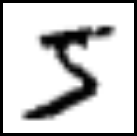
\includegraphics[scale=0.9]{img/5.png}
	\caption{Exemple d'un chiffre de la base MNIST}
\end{figure}


\section{Méthode de recherche}
En utilisant MNIST, l'objectif est de déterminer quelle méthode d'apprentissage permettra d'obtenir un classement avec la meilleure précision tout en gardant un temps d'exécution relativement raisonnable.\\

Cette recherche se place dans un contexte de classement de chiffres afin de reconnaître les numéros étudiants écrits sur une feuille d'examen. Il est donc envisageable d'avoir une erreur lors de la prédiction car le correcteur peut manuellement faire les changements nécessaire dans ce cas. En revanche, plus la précision est importante, plus l'algorithme sera fiable et économisera du temps lors d'une correction. Par ailleurs, le temps d'exécution de l'algorithme n'est pas un facteur majeur mais si celui-ci devient trop conséquent alors la correction assistée sera plus longue qu'une correction manuelle. Dans ce cas, l'algorithme n'est pas pertinent.\\

Deux algorithmes ont été choisis afin de réaliser les tests : K-NN et CART.\\

Le premier, K-NN, a été sélectionné car il permet de tester l'approche paresseuse des classements. La problématique du choix de la valeur de $k$ se résoudra par un choix arbitraire : l'algorithme sera testé avec $k=1$, $k=3$, $k=5$, $k=10$. Les explications précédentes (3.2.2) laissent à penser que $k=10$ sera trop grand, ce qui réduira la précision des résultats. Au contraire, $k=1$ aura une bonne précision mais une marge d'erreur plus grande à cause de l'\textit{overfitting}.\\

Le deuxième algorithme sélectionné est CART. Celui-ci représentera la famille des arbres de décision. L'avantage du traitement des attributs de C4.5 n'est pas exploité avec les données du MNIST car celles-ci sont toutes quantitatives. CART sera par conséquent préféré.\\

Pour répondre à des problèmes de mémoire, le nombre de données d'apprentissage sera réduit 30 000 quant au jeu de test, celui-ci sera réduit à 5000. De plus, une autre série de test sera faite sur un échantillon de 30 000 puis 10 000 d'apprentissage pour 800 de test. Celui-ci sera réalisé dans le but de se rapprocher le plus possible du cas d'une promotion de cent étudiants en moyenne avec chacun un numéro étudiant composé de huit chiffres. Le choix d'un échantillon d'apprentissage plus petit (10 000 observations) et de voir si la perte de précision du au manque de cas est négligeable.\\


Parmi les outils utilisés, Scikit-learn~\cite{scikit-learn} permet d'implémenter les algorithmes cités précédemment. Afin de faciliter son utilisation, il a fallu convertir les fichiers de la base MNIST du format IDX, qui est fait pour les vecteurs et les matrices multidimensionnelles, en format CSV.

\section{Analyse des résultats}
Les tableaux 4.1, 4.2, 4.3 et 4.4 montrent les résultats obtenus suite aux implémentations. La colonne "Précision" correspond au quotient de réussite du classement de l'algorithme. La colonne "Temps" correspond au temps d'exécution du programme, du chargement des données au calcul de la précision. Cette métrique est influencée par les performances de l'ordinateur et de l'allocation donnée au programme. Il faut donc regarder l'ordre de grandeur de celle-ci plutôt que la valeur exacte.\\

Quatre tests ont été réalisés pour chaque algorithme:
\begin{itemize}
\item "Test 1" correspond à 30 000 données d'apprentissage pour 5 000 de test.
\item "Test 2" correspond à 30 000 données d'apprentissage pour 800 de test.
\item Le "Test 3" est composé de 10 000 observations d'apprentissage pour 5 000 de test.
\item "Test 4" est composé de 10 000 observations d'apprentissage pour 800 de test.
\end{itemize}

 
\begin{table}[!h]
\centering
\begin{tabular}{| c | c | c | c | c |}
\hline
 & \multicolumn{2}{c |}{Test 1} & \multicolumn{2}{c |}{Test 2} \\
\hline
k        & Précision             & Temps  & Précision             & Temps\\
\hline
$k = 1$  & 0.9614 ($\pm$ 0.0079) & 1 147s & 0.9614 ($\pm$ 0.0079) & 969s\\
$k = 3$  & 0.9608 ($\pm$ 0.0064) & 1 122s & 0.9608 ($\pm$ 0.0064) & 965s\\
$k = 5$  & 0.9600 ($\pm$ 0.0075) & 1 162s & 0.9600 ($\pm$ 0.0075) & 970s\\
$k = 10$ & 0.9561 ($\pm$ 0.0081) & 1 130s & 0.9561 ($\pm$ 0.0081) & 980s\\
\hline
\end{tabular}
\caption{Résultats de K-NN avec 30 000 observations d'apprentissage}
\end{table}

\begin{table}[!h]
\centering
\begin{tabular}{| c | c | c | c | c |}
\hline
 & \multicolumn{2}{c |}{Test 3} & \multicolumn{2}{c |}{Test 4} \\
\hline
k        & Précision             & Temps  & Précision             & Temps\\
\hline
$k = 1$  & 0.9392 ($\pm$ 0.0146) & 196s & 0.9392 ($\pm$ 0.0146) & 133s\\
$k = 3$  & 0.9395 ($\pm$ 0.0108) & 188s & 0.9395 ($\pm$ 0.0108) & 132s\\
$k = 5$  & 0.9377 ($\pm$ 0.0133) & 194s & 0.9377 ($\pm$ 0.0133) & 134s\\
$k = 10$ & 0.9339 ($\pm$ 0.0161) & 190s & 0.9339 ($\pm$ 0.0161) & 134s\\
\hline
\end{tabular}
\caption{Résultats de K-NN avec 10 000 observations d'apprentissage}
\end{table}

\begin{table}[!h]
\centering
\begin{tabular}{| c | c | c | c |}
\hline
\multicolumn{2}{| c |}{Test 1} & \multicolumn{2}{c |}{Test 2} \\
\hline
Précision             & Temps  & Précision             & Temps \\
\hline
0.8469 ($\pm$ 0.0179) & 54s    & 0.8481 ($\pm$ 0.0157) & 53s\\
\hline
\end{tabular}
\caption{Résultats de CART avec 30 000 observations d'apprentissage}
\end{table}

\begin{table}[!h]
\centering
\begin{tabular}{| c | c | c | c |}
\hline
\multicolumn{2}{| c |}{Test 3} & \multicolumn{2}{c |}{Test 4} \\
\hline
Précision             & Temps  & Précision             & Temps \\
\hline
0.8180 ($\pm$ 0.0150) & 17s    & 0.8125 ($\pm$ 0.0155) & 17s\\
\hline
\end{tabular}
\caption{Résultats de CART avec 10 000 observations d'apprentissage}
\end{table}

\section{Choix de l'algorithme}
Les deux algorithmes peuvent être fondamentalement préférés. L'un permet d'avoir une solution rapidement tandis que l'autre apporte une précision plus fine. Dans le cadre d'une détection de numéros étudiant d'une promotion, qui est composée de 100 étudiants dans ce document, l'algorithme devrait être intégré à une solution qui permettrait de faire plus que reconnaître les chiffres. Que ce soit pour corriger automatiquement ou agréger des exercices entre eux, on peut considérer le fait qu'un tel outil est créé afin d'accélérer la correction des examens papiers. C'est pourquoi avoir un algorithme prenant un peu plus de temps qu'un autre mais qui est plus précis semble plus pertinent pour le correcteur. Dans ce cas, K-NN est l'algorithme à retenir avec $k = 3$. Cette valeur de $k$ a été choisie car c'est avec celle-ci que la précision de l'algorithme est la plus grande tout en prenant en compte l'\textit{overfitting}.